\subsection{Definition and Basic Properties}

Let \(p \geq 3\) be a prime number. Let \(\mathbb{Q}_p\) denote the field of \(p\)-adic numbers, equipped with the \(p\)-adic valuation \(v_p\) and ring of integers \(\mathbb{Z}_p\). A \emph{\(\mathbb{Z}_p\)-lattice} in \(\mathbb{Q}_p^2\) is a free \(\mathbb{Z}_p\)-module of rank \(2\).

Two lattices \(L, M \subset \mathbb{Q}_p^2\) are \emph{homothetic}, written \(L \sim M\), if there exists \(\lambda \in \mathbb{Q}_p^\times\) such that \(L = \lambda M\). The set of vertices of the Bruhat--Tits tree \(T_p\) associated to \(\mathrm{PGL}(2, \mathbb{Q}_p)\) is the set
\[
V(T_p) = \{ [L] \mid L \text{ a \(\mathbb{Z}_p\)-lattice in \(\mathbb{Q}_p^2\)} \}/\sim,
\]
where \([L]\) denotes the homothety class of \(L\).

Two vertices \([L]\) and \([M]\) are joined by an edge if and only if there exist representatives \(L'\) of \([L]\) and \(M'\) of \([M]\) such that \(L' \subset M'\) and the index \([M' : L'] = p\) (i.e., \(M'/L' \cong \mathbb{Z}_p/p\mathbb{Z}_p \cong \mathbb{F}_p\)). This defines a connected graph \(T_p\) which, by the fundamental theorem of Bruhat and Tits, is an infinite \((p+1)\)-regular tree (see \cite{BruhatTits72,Serre80}).

The group \(\mathrm{PGL}(2, \mathbb{Q}_p)\) acts on \(T_p\) by \(g \cdot [L] = [gL]\), transitively on both vertices and edges. The \emph{boundary at infinity} \(\partial T_p\) consists of the equivalence classes of geodesic rays in \(T_p\) and is canonically identified with the projective line
\[
\partial T_p \cong \mathbb{P}^1(\mathbb{Q}_p) = \mathbb{Q}_p \cup \{\infty\}.
\]

To introduce dynamics, fix the distinguished end at \(\infty \in \partial T_p\), corresponding to the ray determined by the standard lattice \(\mathbb{Z}_p e_1 + \mathbb{Z}_p e_2\) with preferred direction along \(e_1\). The \emph{shift operator} \(\sigma_p : T_p \to T_p\) is the unique graph automorphism of \(T_p\) that fixes the end at \(\infty\) pointwise on the corresponding geodesic ray and is induced by the action of the element
\[
g_p = \begin{pmatrix} p & 0 \\ 0 & 1 \end{pmatrix} \in \mathrm{PGL}(2, \mathbb{Q}_p).
\]
Explicitly, on the affine chart \(\mathbb{Q}_p \subset \mathbb{P}^1(\mathbb{Q}_p)\) the induced boundary map is \(\sigma_p(z) = p z\), with \(\sigma_p(\infty) = \infty\).

A \emph{length-\(n\) periodic orbit} on \(T_p\) is a set \(\{v, \sigma_p(v), \sigma_p^2(v), \dots, \sigma_p^{n-1}(v)\}\) consisting of \(n\) distinct vertices such that \(\sigma_p^n(v) = v\) and \(n\) is minimal. (Equivalently, these are the orbits of vertices under the cyclic action generated by \(\sigma_p\).)

\begin{proposition}
There are exactly \(p^n + 1\) periodic orbits of length \(n\) on \(T_p\), one of which is the trivial orbit consisting of the vertex stabilized in the direction of \(\infty\).
\end{proposition}

\begin{proof}
The periodic points of \(\sigma_p^n\) on the boundary \(\partial T_p\) are in bijection with the points of the projective line over the finite ring \(\mathbb{Z}/p^n\mathbb{Z}\), i.e., with \(\mathbb{P}^1(\mathbb{Z}/p^n \mathbb{Z})\). To see this, note that any geodesic ray from a base vertex to a boundary point \(z \in \mathbb{P}^1(\mathbb{Q}_p)\) reduces modulo \(p^n\) to a unique class in \(\mathbb{P}^1(\mathbb{Z}/p^n \mathbb{Z})\). The condition \(\sigma_p^n(z) = z\) lifts precisely to the fixed points of the reduction of \(g_p^n\) modulo \(p^n\), and the cardinality computation is standard:
\[
|\mathbb{P}^1(\mathbb{Z}/p^n \mathbb{Z})| = p^n + 1
\]
(for \(n=1\) this recovers the \(p+1\) points of \(\mathbb{P}^1(\mathbb{F}_p)\); the general case follows by lifting via Hensel's lemma and counting the solutions to the projective equation modulo successive powers of \(p\)). Each such boundary point determines a unique closed geodesic loop of combinatorial length \(n\) on \(T_p\) (by taking the geodesic from the fixed ray at \(\infty\) to the periodic point and back), and distinct points give distinct orbits. The fixed point at \(\infty\) contributes the trivial orbit of length \(1\), completing the count. Full details on the reduction and lifting appear in Serre \cite{Serre80}, Chapter~II, and the original Bruhat--Tits construction \cite{BruhatTits72}.
\end{proof}

\begin{figure}[htbp]
\centering
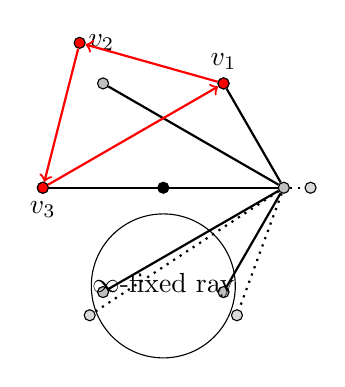
\begin{tikzpicture}[scale=0.85, every node/.style={circle, draw, minimum size=4pt, inner sep=0pt}]
  % Central vertex (base)
  \node[fill=black] (v0) at (0,0) {};
  % Branches for p=5 (degree 6, simplified visualization with 6 directions)
  \foreach \i in {0,60,...,300} {
    \node[fill=gray!50] (v\i) at (\i:1.8) {};
    \draw[thick] (v0) -- (v\i);
  }
  % Highlight a length-3 periodic orbit (using vertices at distance 1--2 from a chosen branch)
  \node[fill=red, label=above:{$v_1$}] (p1) at (60:1.8) {};
  \node[fill=red, label=right:{$v_2$}] (p2) at (120:2.5) {};
  \node[fill=red, label=below:{$v_3$}] (p3) at (180:1.8) {};
  \draw[red, thick, ->] (p1) -- (p2);
  \draw[red, thick, ->] (p2) -- (p3);
  \draw[red, thick, ->] (p3) -- (p1);
  % Additional tree branches (simplified)
  \node[fill=gray!30] (b1) at (0:2.2) {};
  \node[fill=gray!30] (b2) at (240:2.2) {};
  \node[fill=gray!30] (b3) at (300:2.2) {};
  \draw[thick, dotted] (v0) -- (b1);
  \draw[thick, dotted] (v0) -- (b2);
  \draw[thick, dotted] (v0) -- (b3);
  \node[below=2pt] at (0,-0.3) {\(\infty\)-fixed ray};
\end{tikzpicture}
\caption{Bruhat--Tits tree \(T_5\) (simplified local picture) with a highlighted length-3 periodic orbit (red cycle). The full infinite tree extends outward in all \(p+1=6\) directions.}
\label{fig:T5-orbit}
\end{figure}